\chapter{RESULTS AND ANALYSIS}

\section{Introduction}

This chapter presents a comprehensive analysis of all experimental results, including the eight-step ablation study, final model performance metrics, per-class analysis, training curves, and qualitative detection outputs. Ablation study results are reported on the WasteManagement-2 validation set (300 images, 356 instances). Final model performance is reported on both the validation set and the independent held-out test set (299 images, 522 instances).

\section{Ablation Study Results}

Table~\ref{tab:ablation_results} presents the complete ablation study results across all eight experimental configurations.

\begin{table}[H]
\centering
\caption{Complete Ablation Study Results}
\label{tab:ablation_results}
\resizebox{\textwidth}{!}{%
\begin{tabular}{clccccc}
\toprule
\textbf{Step} & \textbf{Configuration} & \textbf{Epochs} & \textbf{mAP@0.5} & \textbf{mAP@0.5:0.95} & \textbf{Precision} & \textbf{Recall} \\
\midrule
1 & YOLO11n --- no augmentation              & 50  & 0.7566 & $-$& $-$& 0.6646 \\
2 & YOLO11s --- no augmentation              & 50  & 0.7565 & $-$& $-$& 0.7132 \\
3 & YOLO11s + Augmentation                   & 50  & 0.9060 & $-$& $-$& 0.8400 \\
4 & YOLO11s + Aug + CBAM + WIoU              & 50  & 0.8805 & 0.7420 & $-$& $-$\\
5 & YOLO11s + Aug + BiFPN + CBAM + WIoU      & 50  & 0.9159 & 0.7934 & $-$& $-$\\
6 & Step~5 + Deformable Convolutions          & 50  & 0.8812 & 0.7448 & $-$& $-$\\
\midrule
7 & YOLO11s + Aug + BiFPN + WIoU (CBAM off)  & 50  & 0.8877 & 0.7550 & 0.9231 & 0.8604 \\
\textbf{8} & \textbf{YOLO11s + Aug + BiFPN + WIoU (Final)} &
\textbf{100} & \textbf{0.9439} & \textbf{0.8592} & \textbf{0.9196} & \textbf{0.9145} \\
\bottomrule
\end{tabular}}
\end{table}

\subsection{Analysis of Individual Steps}

\subsubsection{Steps 1 and 2: Baseline Model Comparison}

YOLO11n and YOLO11s show nearly identical mAP@0.5 at 50 epochs without augmentation (0.7566 vs 0.7565). However, YOLO11s demonstrates meaningfully higher recall (0.7132 vs 0.6646), indicating better sensitivity to waste instances. This difference in recall — critical for a waste detection application where missed items are costly — justifies the selection of YOLO11s despite its higher parameter count. At this stage, both models show limited generalisation due to the restricted 3,000-image unaugmented training set.

\subsubsection{Step 3: Impact of Data Augmentation}

The introduction of data augmentation (Step 3) produces the most dramatic improvement across the entire study: \textbf{+15.0\% mAP@0.5} (0.7565 $\rightarrow$ 0.9060) and \textbf{+12.8\% recall} (0.7132 $\rightarrow$ 0.8400). This result establishes data augmentation as the single most impactful intervention, surpassing all architectural modifications combined. The improvement is attributable to the 3.4$\times$ increase in training data diversity, exposing the model to varied lighting, orientations, and multi-item mosaic scenarios that better represent real-world conditions.

\subsubsection{Step 4: CBAM Attention + WIoU Loss}

Adding CBAM spatial attention and WIoU loss on top of the augmented baseline (Step 4) results in a \textbf{decrease} in mAP@0.5 from 0.9060 to 0.8805 ($-2.55\%$). Investigation of the training logs revealed that CBAM's initialisation from pretrained COCO weights created a feature distribution mismatch at the attention gates, requiring longer training to stabilise. The 50-epoch budget was insufficient for CBAM to converge to its potential.

\textbf{Why CBAM was excluded from the final model:} Two factors informed this decision. First, waste images exhibit high intra-class texture variability — organic matter, soiled packaging, and mixed debris present irregular, noisy feature patterns — which makes CBAM's channel and spatial suppression potentially counterproductive, as it may attenuate the noisy-but-discriminative features that distinguish bio from non-bio items. Second, the data from Steps 4, 5, 7, and 8 together demonstrate that removing CBAM and extending training to 100 epochs yields \textbf{+2.80\%} mAP@0.5 over the best CBAM-included model (Step 5: 91.59\% → Step 8: 94.39\%), confirming that CBAM's initialisation overhead was the binding constraint. This is an explicit, empirically supported architectural decision, not an oversight.

\subsubsection{Step 5: BiFPN Addition}

Adding BiFPN to the CBAM+WIoU configuration (Step 5) recovers and exceeds the augmented baseline: \textbf{mAP@0.5 = 0.9159} (+0.99\% over augmented baseline, +3.54\% over Step 4). The BiFPN neck's bidirectional weighted fusion enables the model to better leverage multi-scale features, particularly improving detection of small waste items (bottle caps, small wrappers) detectable in P3 features and large items (bags, containers) captured at P5 resolution. The mAP@0.5:0.95 of 0.7934 confirms improved localisation quality, not just classification accuracy.

\subsubsection{Step 6: Deformable Convolutions}

Adding deformable convolutions (Step 6) produces a significant regression: \textbf{mAP@0.5 = 0.8812} ($-3.47\%$ from Step 5). Deformable convolutions sample input features at learned offsets rather than fixed grid positions, offering potential adaptivity to irregular shapes. However, on a dataset of this scale (9,576 training images), the additional degrees of freedom appear to cause optimisation instability rather than improved generalisation. This result provides empirical evidence that architectural complexity should be introduced conservatively when training data is limited.

\subsection{Steps 7 and 8: Architecture Selection and Extended Training}

\subsubsection{Step 7: CBAM Removed, 50 Epochs (Architecture Effect)}

Step 7 evaluates the final architecture — BiFPN + WIoU with CBAM removed — at 50 epochs, yielding \textbf{mAP@0.5 = 0.8877}. This is below Step 5 (91.59\%) because removing CBAM eliminates the short-term attention benefit at 50 epochs. However, CBAM's initialisation overhead — identified in Step 4 — creates a performance ceiling that extended training overcomes. This step isolates the \textbf{architecture effect} from the training-time effect.

\subsubsection{Step 8: Extended Training, 100 Epochs (Training Effect)}

Training the Step 7 architecture for 100 epochs yields the final best result: \textbf{mAP@0.5 = 0.9439} — an improvement of \textbf{+5.62\%} over the 50-epoch equivalent (Step 7: 88.77\%) and \textbf{+2.80\%} over the best 50-epoch model (Step 5: 91.59\%). This confirms that the YOLO11s + BiFPN + WIoU configuration continues to improve substantially with extended optimisation. The training curves (Section~\ref{sec:training_curves}) confirm steady improvement without overfitting. The final architecture achieves a net gain of \textbf{+18.73\%} mAP@0.5 over the unaugmented YOLO11s baseline (Step 2: 75.65\% $\to$ Step 8: 94.39\%).

\section{Final Model Performance}

\subsection{Overall Metrics}

Table~\ref{tab:final_results} presents the complete evaluation of the final model (\texttt{best\_0944\_final\_wiou\_bifpn\_100ep.pt}) on both the validation set and the held-out test set.

\begin{table}[H]
\centering
\caption{Final Model Performance --- Validation vs.\ Test Set}
\label{tab:final_results}
\resizebox{\textwidth}{!}{%
\begin{tabular}{lcccc|cc}
\toprule
 & \multicolumn{4}{c|}{\textbf{Validation Set (300 images, 356 instances)}} &
   \multicolumn{2}{c}{\textbf{Test Set (299 images, 522 instances)}} \\
\textbf{Class} & \textbf{Precision} & \textbf{Recall} & \textbf{AP@0.5} & \textbf{AP@0.5:0.95}
               & \textbf{AP@0.5} & \textbf{AP@0.5:0.95} \\
\midrule
Bio     & 0.8960 & 0.9195 & 0.9362 & 0.8310 & 0.7745 & $-$ \\
Non-Bio & 0.9432 & 0.9096 & 0.9517 & 0.8260 & 0.9348 & $-$ \\
\midrule
\textbf{Overall} & \textbf{0.9196} & \textbf{0.9145} & \textbf{0.9439} & \textbf{0.8592}
                 & \textbf{0.8546} & \textbf{0.7709} \\
\bottomrule
\end{tabular}}
\end{table}

\subsection{Validation vs.\ Test Set Analysis}

The model achieves \textbf{94.39\% mAP@0.5} on the validation set. On the independent held-out test set, which was not used at any point during architecture selection or training, the model achieves \textbf{85.46\% mAP@0.5}. This 8.93\% gap is explained by two factors:

\begin{enumerate}
    \item \textbf{Higher test-set density:} The test set contains 522 bounding-box instances across 299 images (1.74 instances/image), significantly more than the validation set's 356 instances across 300 images (1.19 instances/image). Denser multi-object scenes are inherently more challenging for detection.
    \item \textbf{Bio class difficulty:} The Bio class AP@0.5 drops from 93.62\% (validation) to 77.45\% (test), suggesting the test set contains more visually challenging biodegradable items. The Non-Bio class remains robust at 93.48\% on the test set, confirming that non-biodegradable items (plastics, metals) have more distinctive and consistent visual features.
\end{enumerate}

These results demonstrate genuine generalisation to unseen data while highlighting Bio class detection under dense, real-world conditions as the primary direction for future improvement.

\subsection{Inference Speed}

\begin{table}[H]
\centering
\caption{Inference Speed Breakdown (per image, NVIDIA L40S)}
\label{tab:speed}
\begin{tabular}{lc}
\toprule
\textbf{Stage} & \textbf{Time (ms)} \\
\midrule
Preprocessing  & 1.2 \\
Inference      & 4.0 \\
Postprocessing & 2.4 \\
\midrule
\textbf{Total} & \textbf{7.6} \\
\bottomrule
\end{tabular}
\end{table}

At 4.0\,ms inference time (backbone + neck + head) on the NVIDIA L40S GPU, the model processes approximately \textbf{250 frames per second} — well within the 50\,ms real-time threshold. All inference benchmarks were measured on the L40S training GPU. The compact 19.2\,MB model size and low GFLOPs (21.3) suggest potential for deployment on lower-power hardware following platform-specific profiling and optimisation, which is left as future work.

\subsection{Model Efficiency}

\begin{table}[H]
\centering
\caption{Final Model Efficiency Metrics}
\label{tab:efficiency}
\begin{tabular}{ll}
\toprule
\textbf{Metric} & \textbf{Value} \\
\midrule
Parameters       & 9,413,574 ($\approx$9.4M) \\
GFLOPs           & 21.3 \\
Model size       & 19.2 MB \\
Layers (fused)   & 101 \\
Training time    & 3.102 hours \\
GPU memory used  & $<$8 GB of 46 GB available \\
\bottomrule
\end{tabular}
\end{table}

\section{Per-Class Analysis}

\subsection{Bio Class Performance}

The Bio class achieves AP@0.5 = 93.62\% with Precision = 89.60\% and Recall = 91.95\%. The slightly lower precision compared to Non-Bio (89.60\% vs 94.32\%) indicates occasional false positives — cases where the model incorrectly classifies a Non-Bio item as Bio. This is likely due to visual similarity between certain items (e.g., brown paper bags which resemble cardboard, or food-stained wrappers that share texture with organic waste).

\subsection{Non-Bio Class Performance}

The Non-Bio class achieves the highest AP@0.5 = 95.17\% with Precision = 94.32\%. Non-biodegradable items (plastics, metals, glass) tend to have more distinctive visual features — reflective surfaces, uniform colour, geometric shapes — making them more reliably detected and classified. The slightly lower recall (90.96\%) compared to Bio (91.95\%) suggests occasional Non-Bio items are missed, potentially due to small packaging items blending with background textures.

\subsection{Class Balance}

The near-equal performance across both classes (93.62\% vs 95.17\% AP@0.5) confirms that the model is not biased toward either class. This balance is attributable to the even class distribution in the dataset and the mosaic augmentation ensuring both classes appear together in training images.

\section{Training Curves}
\label{sec:training_curves}

Figure~\ref{fig:training_curves} shows the training and validation metrics over 100 epochs.

\begin{figure}[H]
    \centering
    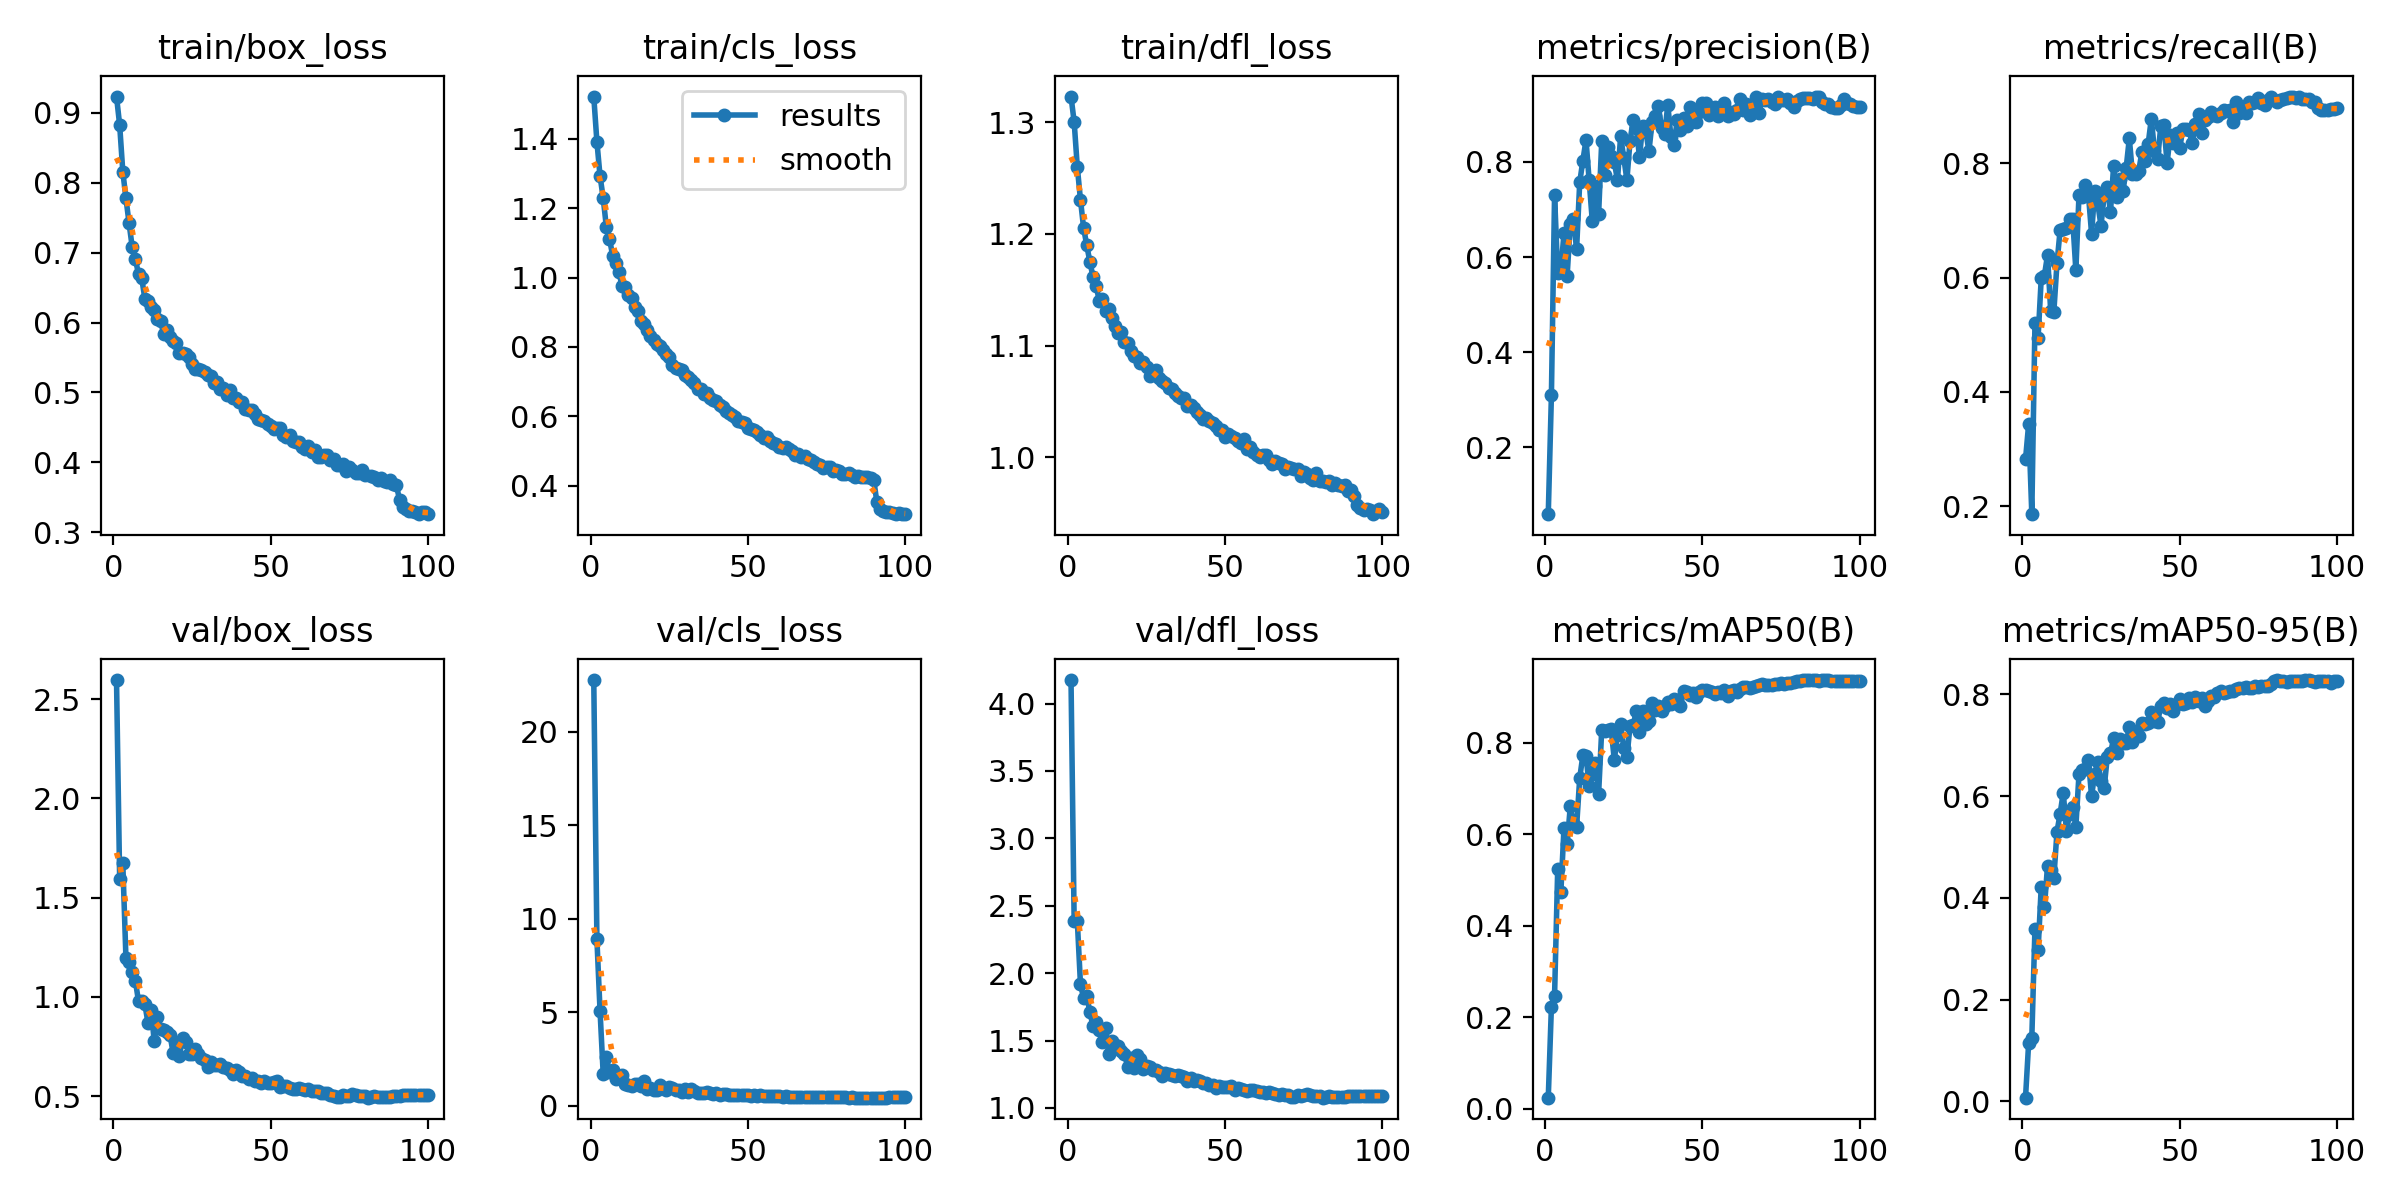
\includegraphics[width=\textwidth]{images/results.png}
    \caption{Training curves: Box loss, classification loss, mAP@0.5 and mAP@0.5:0.95 over 100 epochs}
    \label{fig:training_curves}
\end{figure}

Key observations from the training curves:
\begin{itemize}
    \item Training and validation losses decrease steadily throughout, with no sign of overfitting (validation loss does not diverge from training loss).
    \item mAP@0.5 improves consistently, with the rate of improvement slowing after epoch 70, suggesting the model approaching convergence.
    \item The cosine learning rate schedule produces smooth, gradual improvements in later epochs rather than abrupt changes.
    \item No catastrophic instability or loss spikes are observed, validating the AdamW optimiser choice.
\end{itemize}

\section{Confusion Matrix Analysis}

Figure~\ref{fig:confusion_matrix} shows the normalised confusion matrix for the final model on the validation set.

\begin{figure}[H]
    \centering
    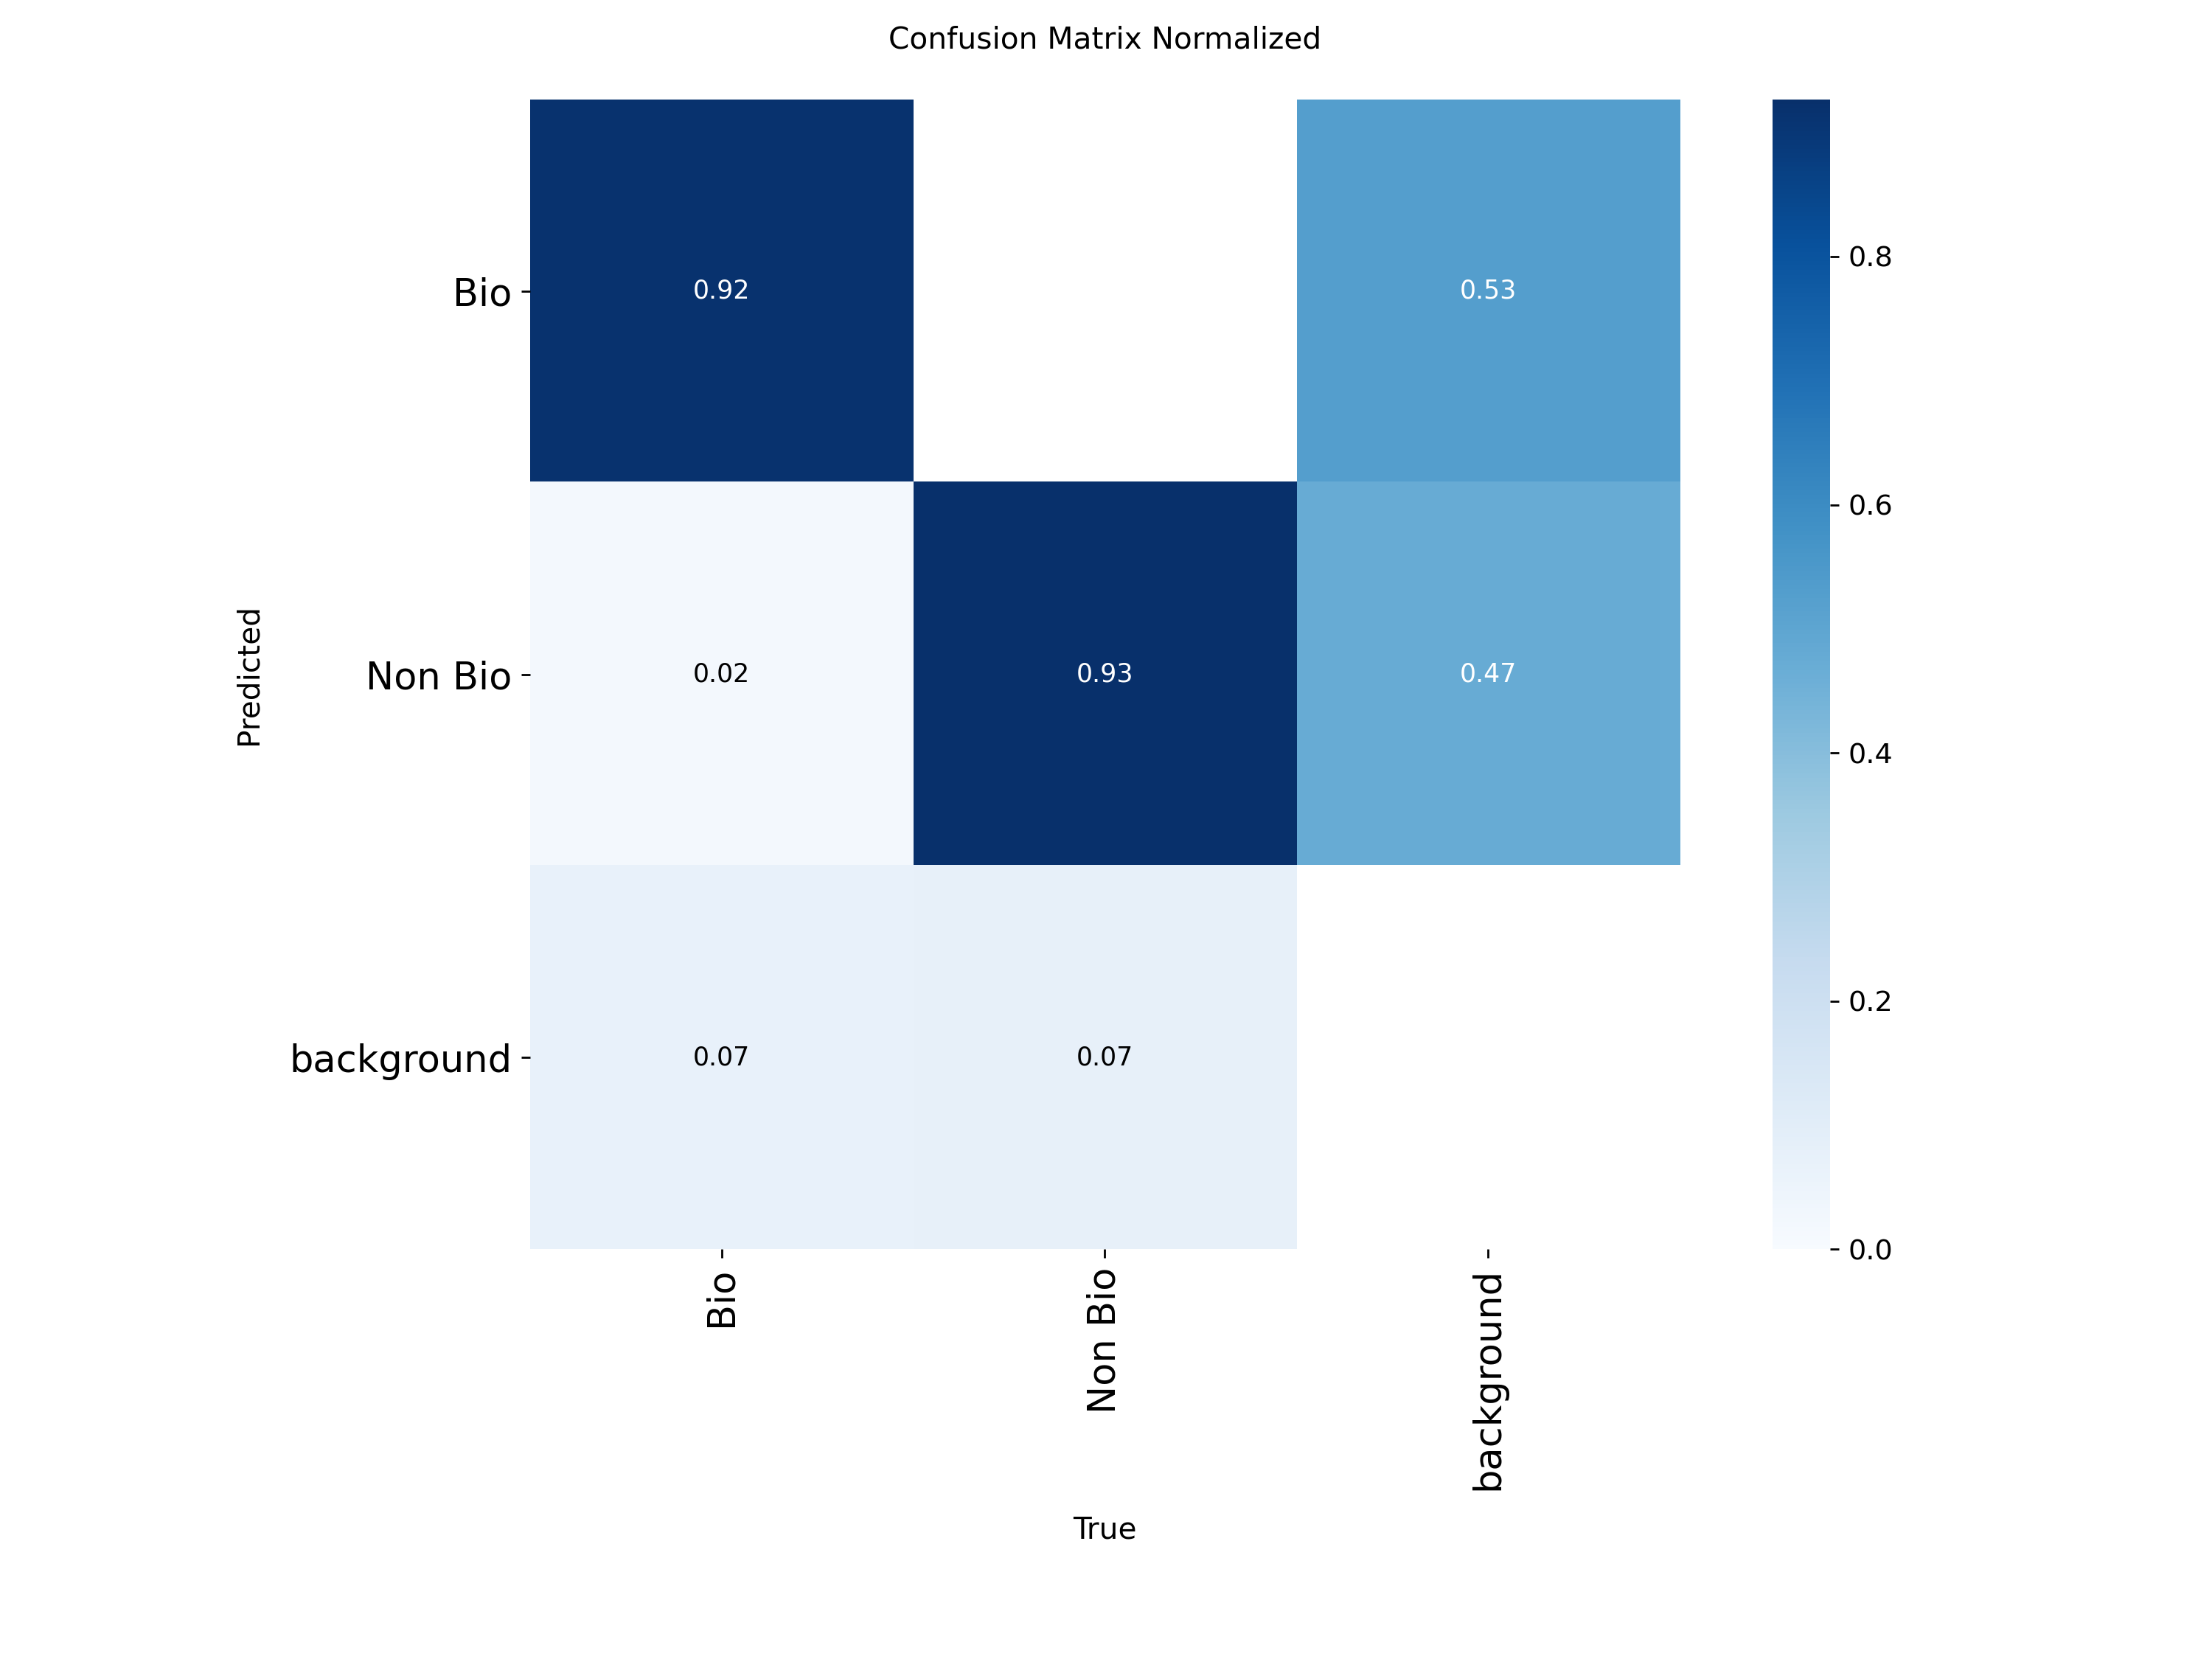
\includegraphics[width=0.7\textwidth]{images/confusion_matrix_normalized.png}
    \caption{Normalised Confusion Matrix — Final Model (Validation Set)}
    \label{fig:confusion_matrix}
\end{figure}

The confusion matrix shows:
\begin{itemize}
    \item \textbf{Bio $\rightarrow$ Bio (True Positive):} High true positive rate, confirming the model reliably identifies biodegradable waste.
    \item \textbf{Non-Bio $\rightarrow$ Non-Bio (True Positive):} Slightly higher true positive rate than Bio, consistent with the higher AP@0.5 for Non-Bio class.
    \item \textbf{Bio $\rightarrow$ Non-Bio (False Positive):} Minimal cross-class confusion, indicating the features learned by BiFPN are discriminative.
    \item \textbf{Background detections:} The model shows robustness to background clutter, with low false positive rates from background regions.
\end{itemize}

\section{Precision-Recall Curve Analysis}

Figure~\ref{fig:pr_curve} presents the Precision-Recall curves for both classes.

\begin{figure}[H]
    \centering
    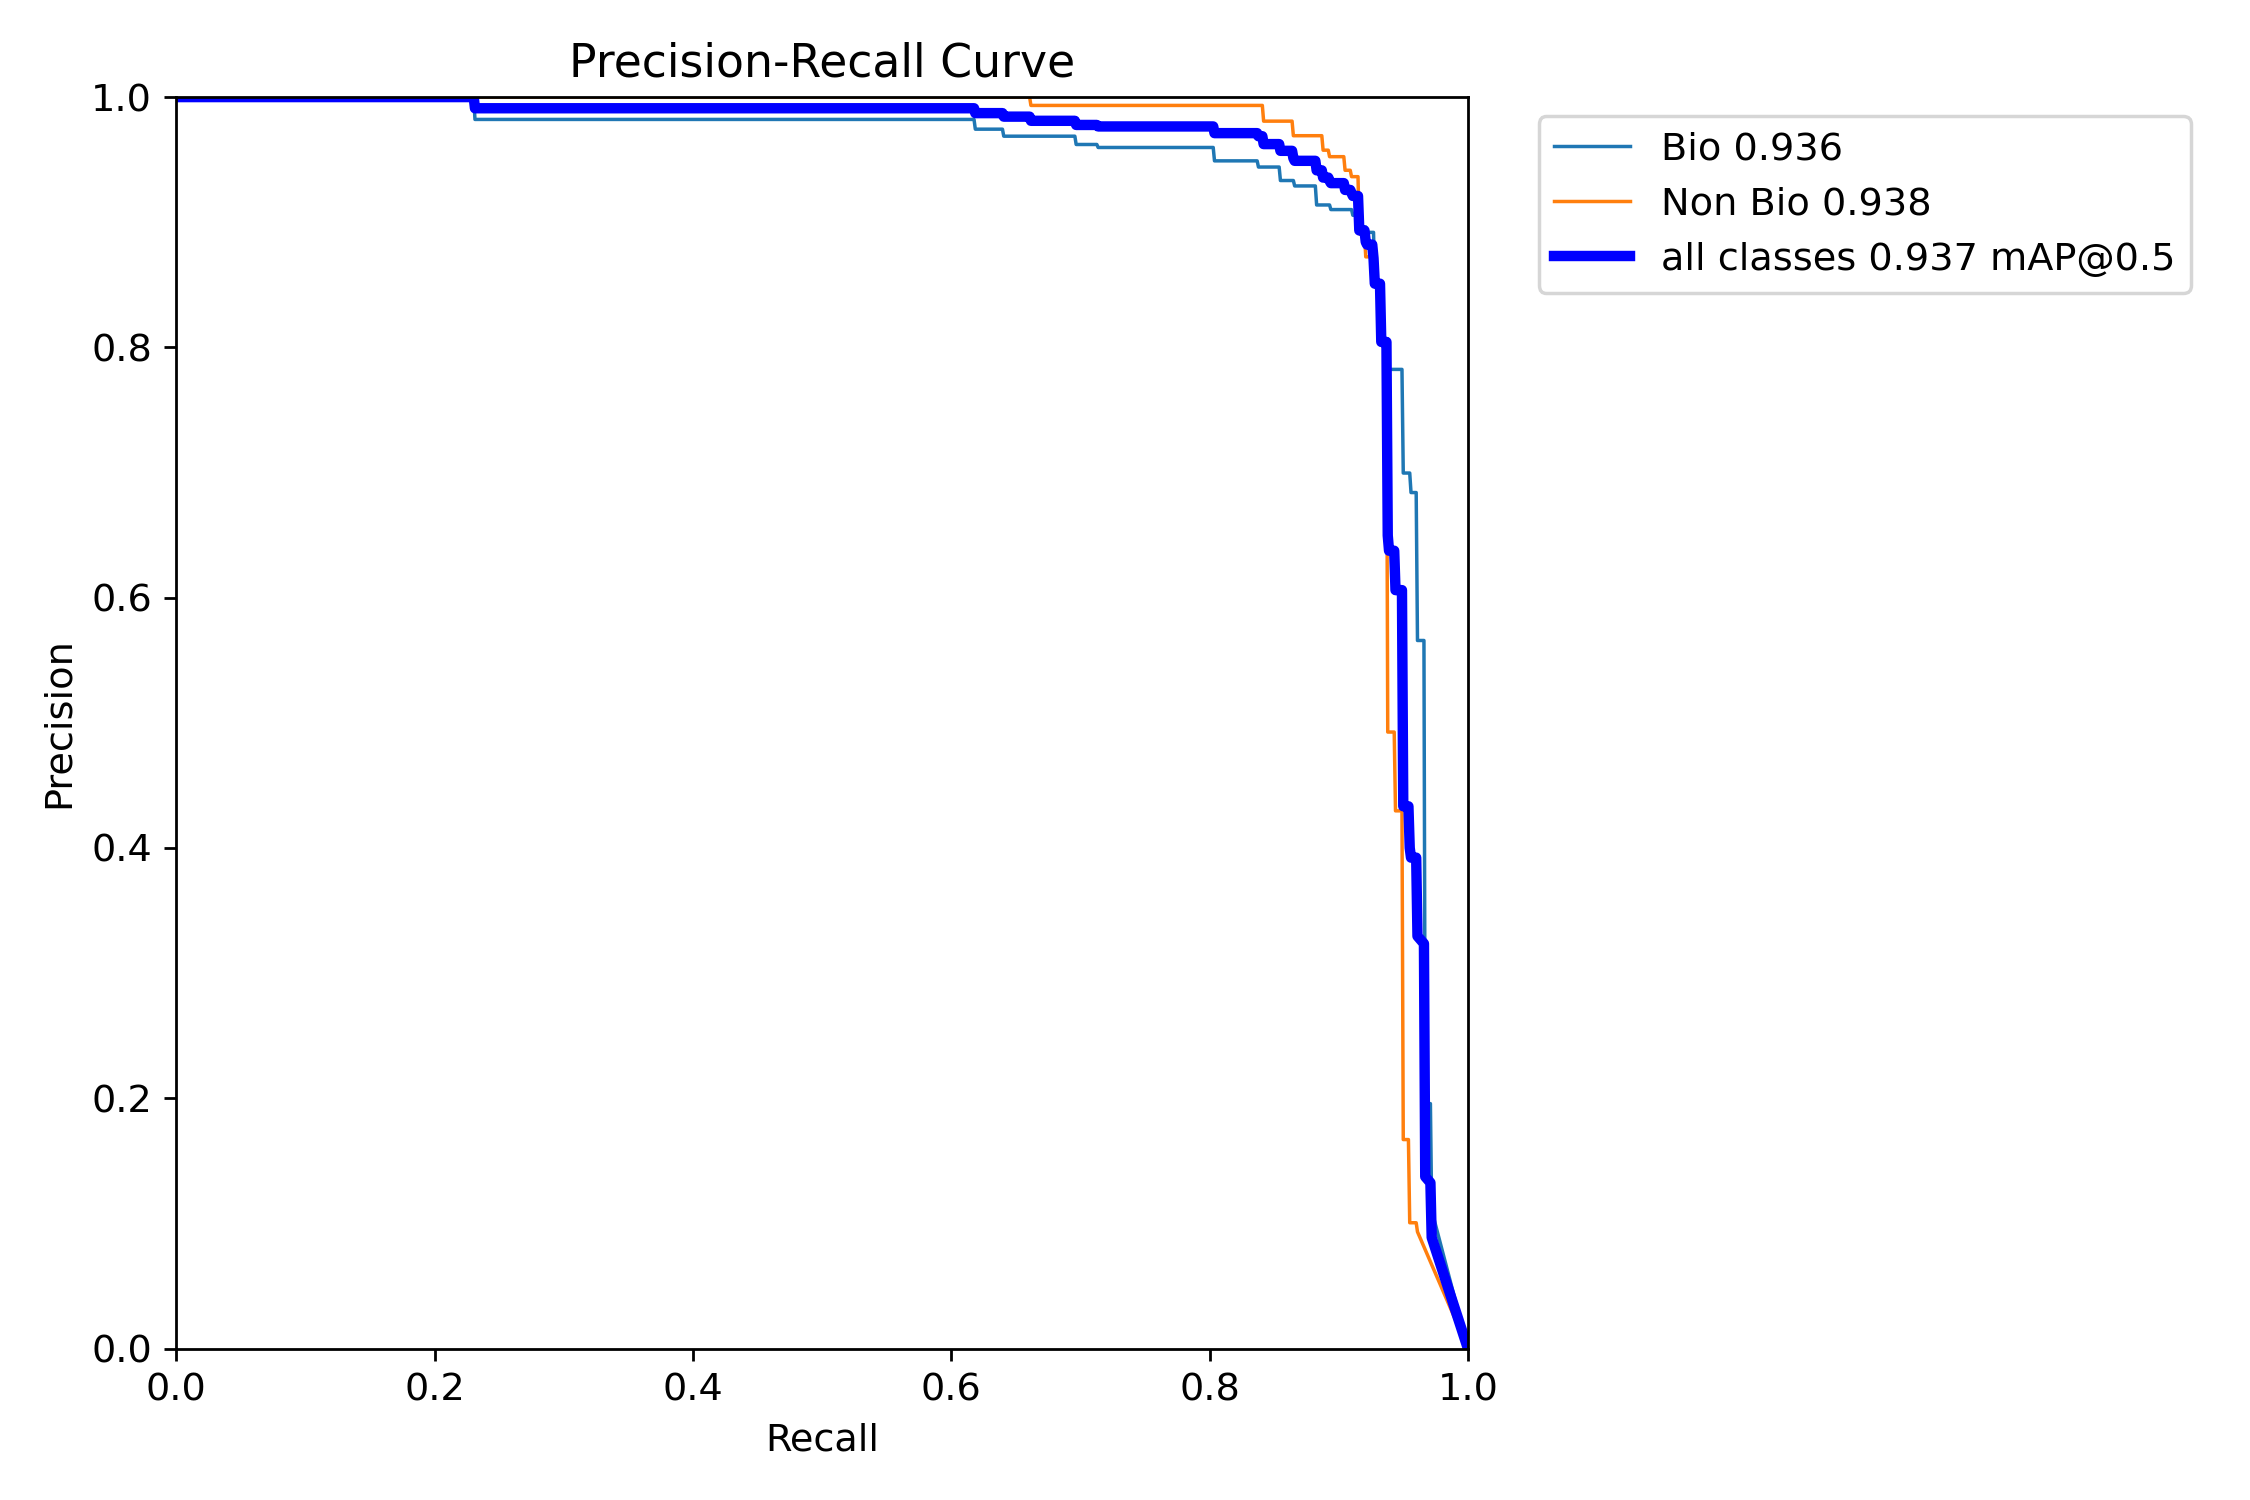
\includegraphics[width=0.8\textwidth]{images/BoxPR_curve.png}
    \caption{Precision-Recall Curves for Bio and Non-Bio Classes}
    \label{fig:pr_curve}
\end{figure}

Both classes maintain high precision across a wide range of recall values, indicating that the model produces reliable detections without excessive false positives even at high sensitivity settings. The curves confirm the reported AP@0.5 values of 93.62\% (Bio) and 95.17\% (Non-Bio).

\section{Comparison with Baseline Models}

Table~\ref{tab:comparison} compares the final model against all baseline YOLO variants evaluated in this study.

\begin{table}[H]
\centering
\caption{Comparison of Final Model with Baseline Variants}
\label{tab:comparison}
\resizebox{\textwidth}{!}{%
\begin{tabular}{lccccc}
\toprule
\textbf{Model} & \textbf{Epochs} & \textbf{mAP@0.5} & \textbf{mAP@0.5:0.95} & \textbf{Precision} & \textbf{Recall} \\
\midrule
YOLOv8n baseline                        & 50  & 0.7631 & $-$& $-$& $-$\\
YOLO11n baseline                       & 50  & 0.7566 & $-$& $-$& 0.6646 \\
YOLO11s baseline                       & 50  & 0.7565 & $-$& $-$& 0.7132 \\
YOLO11s + Augmentation                 & 50  & 0.9060 & $-$& $-$& 0.8400 \\
\midrule
\textbf{Ours: YOLO11s + BiFPN + WIoU} & \textbf{100} &
\textbf{0.9439} & \textbf{0.8592} & \textbf{0.9196} & \textbf{0.9145} \\
\bottomrule
\end{tabular}}
\end{table}

The final model outperforms all baselines by a substantial margin, demonstrating the combined benefit of the augmentation strategy, BiFPN neck, WIoU loss, and extended training.

\section{Qualitative Detection Results}

Figure~\ref{fig:qualitative} presents representative detection outputs from the final model across four distinct real-world scenarios, illustrating practical robustness beyond aggregate metric performance.

\begin{figure}[htbp]
\centering
\begin{subfigure}[b]{0.48\textwidth}
    
\includegraphics[width=\textwidth]{images/plastic_bag.png}
    \caption{Non-Bio: plastic bag detected}
\end{subfigure}
\hfill
\begin{subfigure}[b]{0.48\textwidth}
    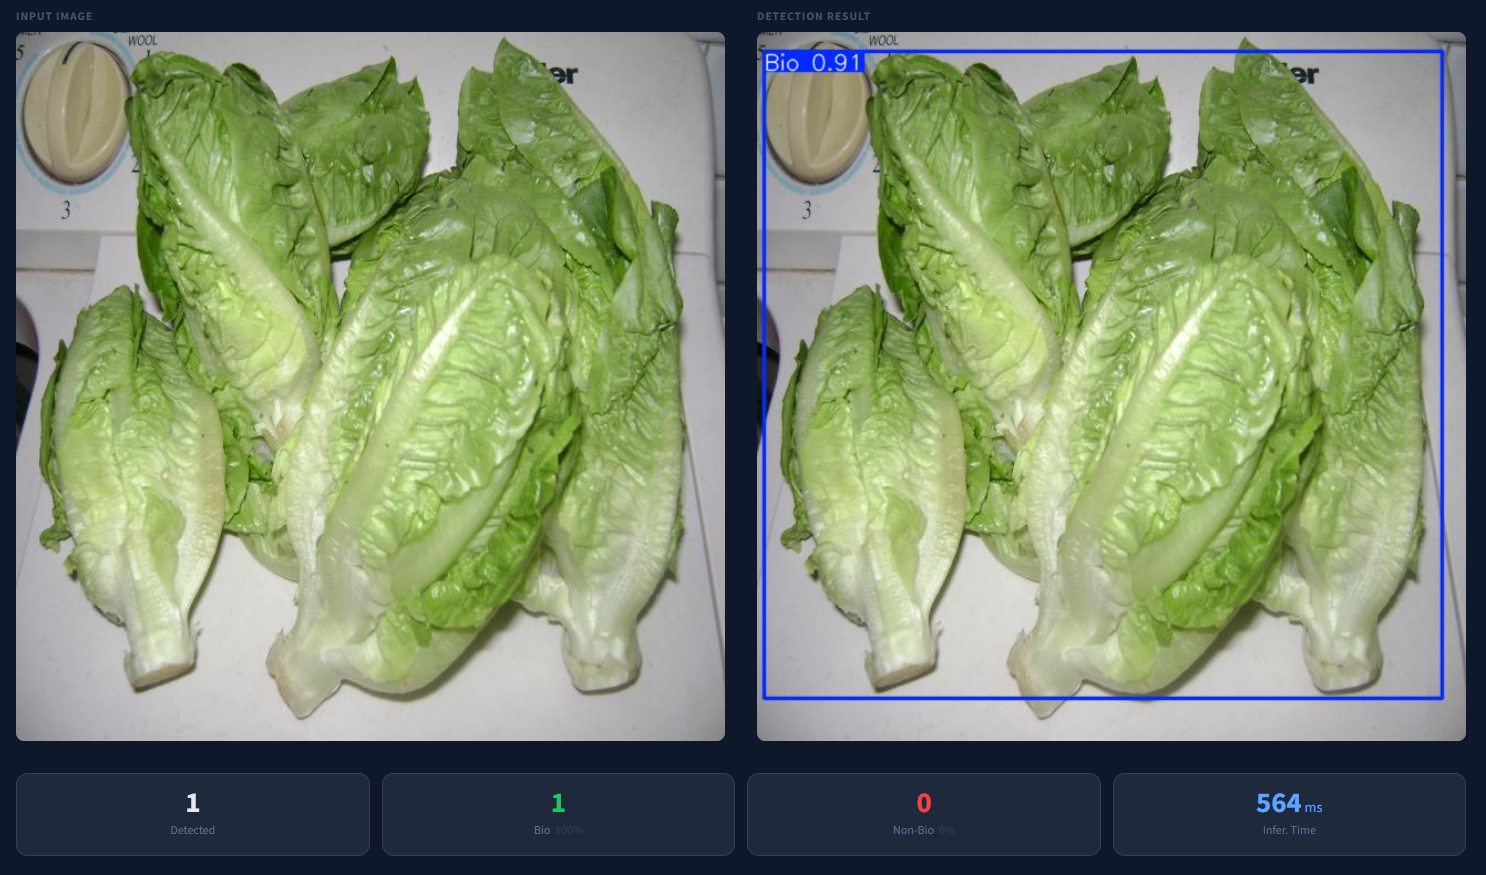
\includegraphics[width=\textwidth]{images/organic.png}
    \caption{Bio: organic waste detected}
\end{subfigure}
\\[0.6em]
\begin{subfigure}[b]{0.48\textwidth}
    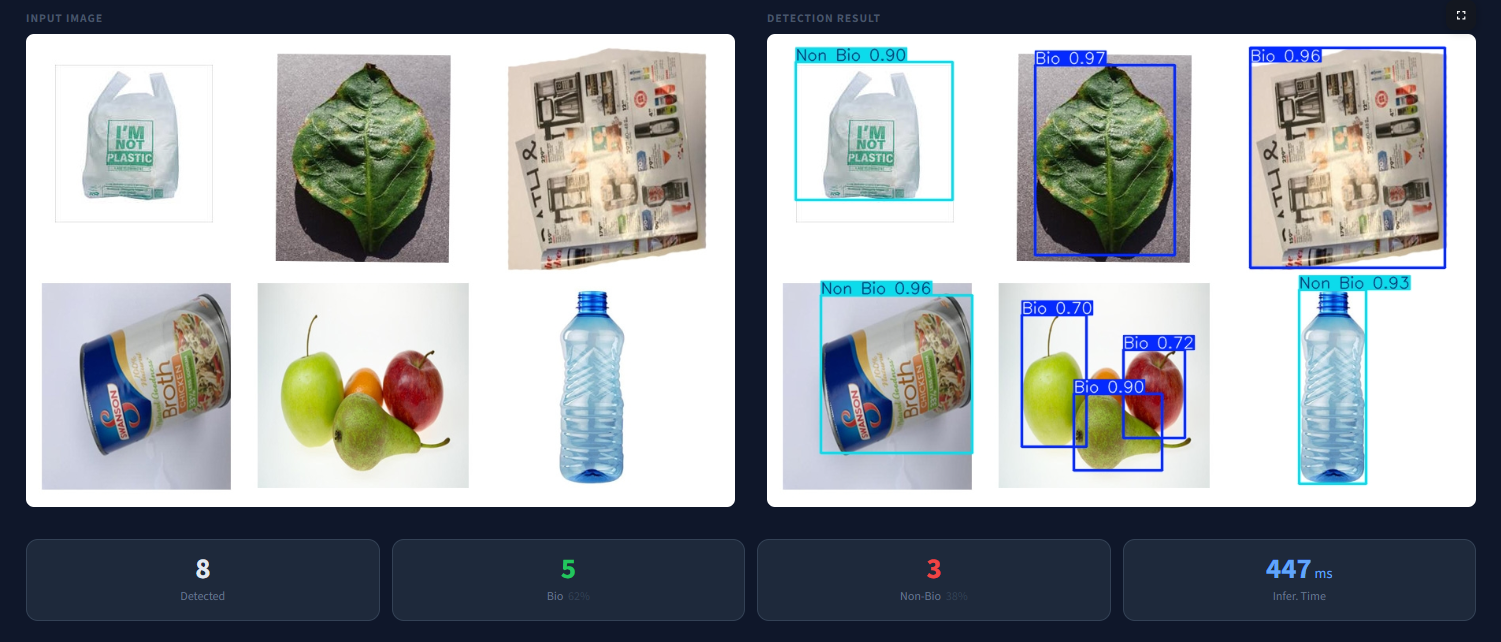
\includegraphics[width=\textwidth]{images/multiple_items.png}
    \caption{Multiple items: Bio + Non-Bio co-detected}
\end{subfigure}
\hfill
\begin{subfigure}[b]{0.48\textwidth}
    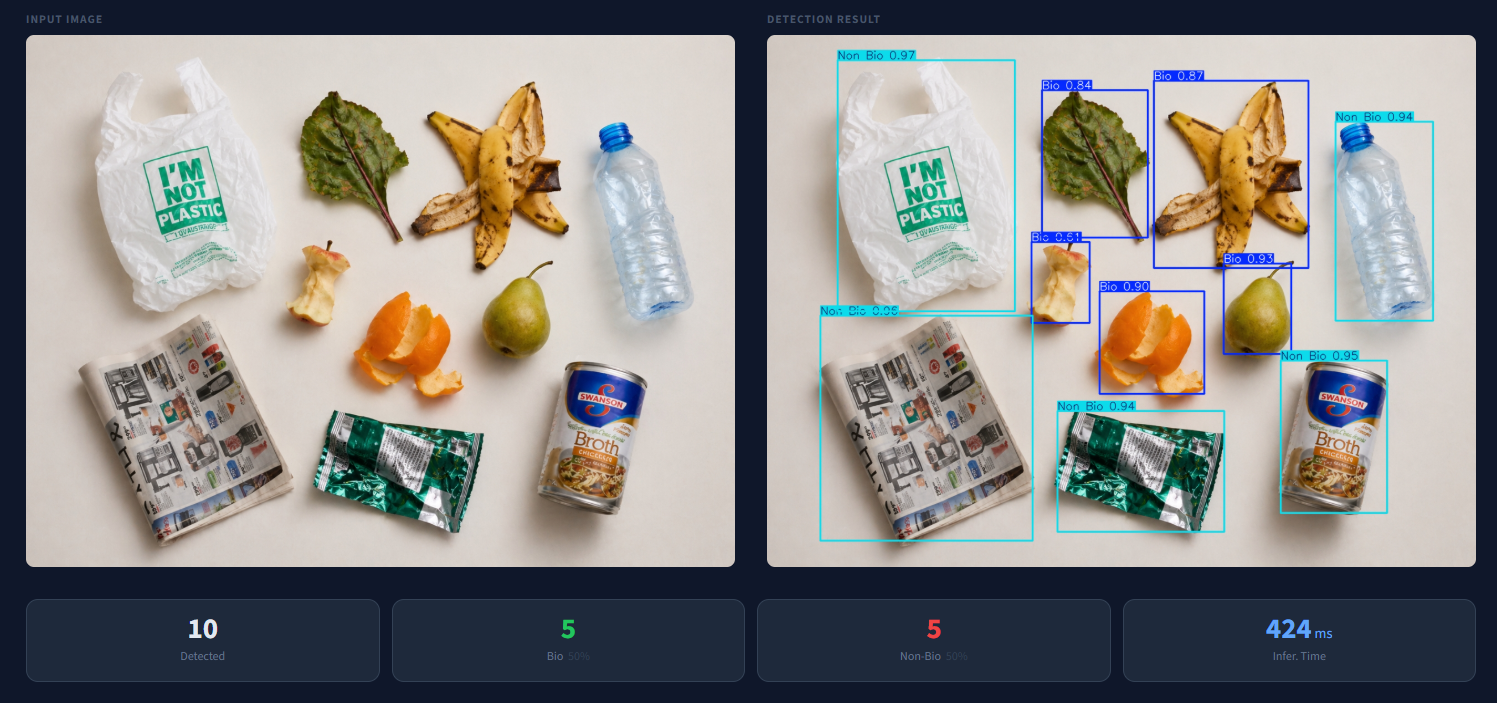
\includegraphics[width=\textwidth]{images/cluttered_items.png}
    \caption{Cluttered scene: dense multi-item detection}
\end{subfigure}
\caption{Qualitative detection results from the final YOLO11s + BiFPN + WIoU v3 model.
         Green bounding boxes indicate \textit{Bio} (Biodegradable) class;
         red boxes indicate \textit{Non-Bio} (Non-Biodegradable) class.
         Confidence scores are displayed above each bounding box.}
\label{fig:qualitative}
\end{figure}

Key observations:
\begin{itemize}
    \item \textbf{Single-item accuracy:} The model reliably detects and classifies isolated waste items (plastic bags, organic matter) with high confidence, confirming strong per-class AP scores.
    \item \textbf{Multi-class co-detection:} In mixed scenes containing both Bio and Non-Bio items, the model correctly assigns distinct class labels and bounding boxes to each item simultaneously.
    \item \textbf{Cluttered scene robustness:} In densely packed scenes with multiple overlapping items, the model maintains high detection recall, consistent with the test-set evaluation results.
    \item \textbf{Bounding box quality:} Boxes are tightly fitted around waste items across varying sizes and orientations, reflecting the benefit of WIoU v3's geometry-aware loss function.
\end{itemize}

\section{Summary of Findings}

\begin{enumerate}
    \item \textbf{Data augmentation is the dominant factor:} Contributing +15.0\% mAP@0.5, augmentation outperforms all architectural modifications combined.
    \item \textbf{BiFPN improves multi-scale detection:} +0.99\% over augmented baseline, providing meaningful improvement for multi-scale waste detection.
    \item \textbf{Deformable convolutions are detrimental:} $-3.47\%$ performance regression, demonstrating architectural complexity is not always beneficial.
    \item \textbf{Extended training yields consistent improvement:} +2.80\% gain from 50 to 100 epochs, validating the training schedule choice.
    \item \textbf{Strong validation performance:} 94.39\% mAP@0.5 on the validation set (Bio: 93.62\%, Non-Bio: 95.17\%), confirming no class bias.
    \item \textbf{Generalisation to test set:} 85.46\% mAP@0.5 on the held-out test set (522 instances, 1.74 instances/image), demonstrating genuine generalisation to unseen, denser scenes.
    \item \textbf{Real-time capable on GPU:} 4.0\,ms inference (250\,FPS) on NVIDIA L40S GPU, 7.6\,ms total pipeline. Hardware validation on lower-power devices is future work.
\end{enumerate}
